%\begin{document}
%\title{Electronica III \\
%Trabajo Practico de Laboratorio N 1}
%
%\author{Martin Rodriguez Turco\\
% Juan Martin Laguinge\\
% Tobias Scala\\
% Guido Panaggio}
%\date{5 de Septiembre de 2018}
%
%\begin{Large}
%\maketitle
%\end{Large}
%
%\input{Ejercicios/Ejercicio1.tex}
%\input{Ejercicios/Ejercicio2.tex}
%\input{Ejercicios/Ejercicio3.tex}
%\input{Ejercicios/Ejercicio4.tex}
%\input{Ejercicios/Ejercicio5.tex}
%\input{Ejercicios/Ejercicio6.tex}
%\end{document}
% Doğancan Özturan 
% Creative Commons Attribution-ShareAlike 4.0 International License.

\documentclass[a4paper]{report}
\usepackage[tmargin=4cm, bmargin=2.50cm]{geometry} %margin of the document
\usepackage{graphicx} % for the images on the document
\usepackage[utf8]{inputenc}
\setcounter{secnumdepth}{3} % for the visualization of the toc
\setcounter{tocdepth}{3} % for the visualization of the toc
\usepackage[linktoc=all]{hyperref} % for clickable toc
\usepackage{setspace}
\usepackage{color}
%\usepackage{tocloft}

\onehalfspacing

\begin{document}
\begin{titlepage}

\newcommand{\HRule}{\rule{\linewidth}{0.5mm}} % a new command for the horizontal lines, change thickness
\center % Center everything

%	LOGO SECTION

\includegraphics[scale=0.25, keepaspectratio]{logo.jpg}\\[0.5cm] % Logo of the university

%	HEADING SECTIONS
\textsc{\LARGE Galactic Republic University}\\[0.5cm] % Name of the university
\textsc{\Large Faculty of Galactic Sciences}\\[0.5cm] % Name of the faculty
\textsc{\Large Department of Jedi Science}\\[0.5cm] % Name of the department
\textsc{\Large Fall}\\[0.3cm] % Term 
\textsc{\large Advanced Light Saber}\\[2.5cm] % Course Title

%	TITLE SECTION
\HRule \\[0.4cm]
{\LARGE  A brief History of techniques in Light Saber}\\[0.2cm] % Title of the document
\HRule \\[0.4cm]

%	AUTHOR SECTION
\begin{minipage}{0.4\textwidth}
\begin{flushleft} \large
\emph{Author:}\\
Luke \textsc{Skywalker} % Name
\end{flushleft}
\end{minipage}
~
\begin{minipage}{0.4\textwidth}
\begin{flushright} \large
\emph{Instructor:} \\
Obi-Wan \textsc{Kenobi} % Supervisor's Name
\end{flushright}
\end{minipage}\\[6cm]

%	DATE SECTION
{\large \today}\\[3cm] % Date
 
\vfill % Fill the rest of the page with whitespace

\end{titlepage}

% Table of Contents

\tableofcontents
 
\newpage

%List of figures and tables
\phantomsection
\listoffigures
\addcontentsline{toc}{section}{List of Figures} 


\phantomsection
\listoftables 
\addcontentsline{toc}{section}{List of Tables} 
\newpage


% Abstract
\phantomsection

\newpage

\clearpage
\chapter{NotGATE}
\subsection{Objetivo}
Implementar de dos manera diferente una compuerta \emph{NOT} utilizando transistores de tecnologia \emph{BJT}

\begin{center}
Tabla de verdad NOT GATES
	\begin{center}
		\begin{tabular}{|c|c|}
					\hline
					\textbf{INPUT} & \textbf{OUTPUT} \\
					\hline
					0  &  1\\
					\hline
					1  & 0\\
					\hline
				\end{tabular}
	\end{center}
\end{center}
			
			
https://www.youtube.com/watch?v=XpN0IQMHo7k
%\documentclass{report}
%%Libreries needed
%
%%Needed to use diagbox that make the \ in the table
%\usepackage{diagbox}
%%Needed to set the edge of the document
%\usepackage{vmargin}
%%Para las flechitas de la tabla
%\usepackage{amssymb}

%%Beginning of the document
%\begin{document}
%\setpapersize{A4}
%\setmargins{2.5cm}   % Left edge
%{1.5cm}                      % Superior edge
%{12cm}                       % Text width
%{20cm}                   	   % Height of the text
%{10pt}                        % Height of the headers
%{1cm}                         % Space between the text and the headers
%{0pt}                          % Height of the foot of page
%{2cm}                         % Space between the tax and the foot of page
\chapter{Noise Margin}
%\stepcounter{chapter}

Se realizo una comparación entre el cambio de márgenes de ruido causados por la combinación entre las compuertas 74HC02 y 74LS02 y, entre 74HCT02 y 74LS02. Pero primero expondremos una breve síntesis entre las diferencias esenciales entre ellas.
La primera diferencia esencial entre ellas es el transistor interno que usan, las compuertas HCT y HC es un transistor de efecto de campo, CMOS, mientras que las compuertas LS utilizan un transistor bipolar, BJT. Debido a esto la compuerta LS van a requerir mayor potencia que las demás, pero van a tener tiempos más rápidos mientras que las HCT y HC a pesar de requerir un mayor tiempo van a tener un bajo consumo de tiempo. Por último, la diferencia esencial entre la HCT y la HC es que una posee una salida más compatible para la alimentación de las LS, de forma tal que una combinación de HC y LS va a tener problemas dado por las diferencias de salida del HC y la entrada requerida en LS mientras que para la HCT esto no sucede.
Del datasheet se pueden obtener los siguientes valores en donde $V_{IHmin}$ es la mínima tensión de entrada que la compuerta reconoce como High,$V_{ILmax}$ es la máxima tensión de entrada que la compuerta reconoce como Low,$V_{OHmin}$ es la mínima tensión de salida dada por la compuerta dado que esta en High y $V_{OLmax}$ es la máxima tensión de salida dada por la compuerta dado que esta en Low.\\
\begin{center}
	\begin{table}[!h]
		\begin{center}
		\caption{Datasheet}
			\begin{tabular}{|c|c|c|c|c|}
				\hline
				\textbf{Integrado digital} & \textbf{$V_{IHmin}$} & \textbf{$V_{OHmin}$} & \textbf{$V_{ILmax}$}& \textbf{$V_{OLmax}$}\\
				\hline
				\textbf{74HC02} & 2,4 V & 4,32 V & 2,1 V & 0,15 V\\
				\hline
				\textbf{74HCT02} & 2 V & 4,32 V & 0,8 V & 0,15 V\\	
				\hline
				\textbf{74LS02} & 2 V & 2,7 V & 0,8 V & 0,5 V\\
				\hline
			\end{tabular}
		\end{center}
	\end{table}
\end{center}
Luego de la combinación  en donde un circuito alimenta al otro, se obtuvieron los siguientes valores:\\
\FloatBarrier
\begin{center}
	\begin{table}[!h]
	\begin{center}
		\caption{Valores Experimentales}
			\begin{tabular}{|c|c|c|c|c|}
				\hline
				\textbf{Circuitol} & \textbf{$V_{IHmin}$} & \textbf{$V_{OHmin}$} & \textbf{$V_{ILmax}$}& \textbf{$V_{OLmax}$}\\
				\hline
				\textbf{$HC \dashrightarrow LS$} & 2,5 V & 4,1 V & 2,3 V & 0,15 V\\
				\hline
				\textbf{$LS \dashrightarrow HC$} & 1,1 V & 2,51 V & 0,94 V & 0,02 V\\
				\hline
				\textbf{$HCT \dashrightarrow LS$} & 1,2 V & 4 V & 1 V & 0,15 V\\
				\hline
				\textbf{$LS \dashrightarrow HCT$} & 1,1 V & 2,4 V & 0,950 V & 0,02 V\\
				\hline
			\end{tabular}
		\end{center}
	\end{table}
\end{center}
\FloatBarrier
Cabe mencionar que, durante la experiencia, las mediciones se realizaron con una señal cuadra de amplitud 20 mV en donde se fue variando el offset para poder obtener los valores medidos y que se uso una protobaord con lo cual los valores pueden presentar ligeros errores. Además, hay que mencionar que durante la experiencia se encontró un intervalo de 1,1 V a 0,9 V el cual dependiendo del pasado se tenía, para obtener un estado de Low o High en la compuerta LS dado que fuera alimentada con una HC y que en la HCT el intervalo era de 1 V a 0,95 V. Esto se puede deber a que la compuerta HC/HCT no podía darle la corriente necesaria para la polarización del transistor BJT de la LS causando que no funcione correctamente.Se debe mencionar que en ese intervalo devolvía High dado que viniera del estado High y Low si venia del estado Low.\\
Para el cálculo del fan-out se obtuvo de la datasheet que los componentes 74HC02 y 74HCT02 tenían la siguiente corriente de entrada, $I_i= \pm 1 \mu A$ y una corriente de salida, $I_o= \pm 4 mA$ mientras que para la 74LS02 los valores fueron $I_i= \pm 20 \mu A$ para el High mientras que $I_i= \pm -0,4 mA$ para el Low y $I_o= \pm -0,4 mA$ para el High y$I_o= \pm 8 mA$ para el Low respectivamente.
\\
Luego utilizando la fórmula de fan-out, $fan-out=|I_o/I_i|$ en donde se realiza tanto para el estado High como el Low y uno se queda con el valor más chico. Entonces obtenemos que para las compuestas HC y HCT se le pueden alimentar hasta 10 LS mientras que para la LS podemos alimentar hasta 400 HC/HCT.\\
Podemos concluir, que la conexión entre elementos de distintos tipo siempre puede acarrear problemas, pero para evitar un cambio drástico en el margen de Ruido es necesario utilizar compuertas tales que sean compatibles entre si como la HCT y la LS pero se debe tener en cuenta que las diferencias dadas en las tensiones de salida son debidas a la salida que puede dar el elemento con lo cual a menos que posean salidas iguales siempre se van a ver diferentes. Por ultimo, debido a que los valores de las tensiones de input son iguales en el LS y HCT el orden en el cual se conectan es casi indistinto mientras que para la HC por las diferencias de estas el orden cambia drásticamente la salida.\\
%\end{document}
\chapter{Tabla de Verdad}

%Ejemplo de Karnaugh
EJEMPLO DE MAPA DE KARNAUGH
 \begin{center}
 \begin{Karnaughvuit}
		\minterms{1,3,2,5}
        \maxterms{0,4,7,6}
       	\implicant{1}{5}{green}
       	\implicant{3}{2}{orange}
       	%\implicant{1}{3}{red}
\end{Karnaughvuit}
\end{center}
\chapter{74HC02}
%\stepcounter{chapter}

\begin{center}
	\begin{table}[h!] 	%With the [h!] we told the document to have the table lock on this position and not to move it
		\begin{center}
		\caption{Mediciones Realizadas}
			\begin{tabular}{|c|c|c|c|}
				\hline
				\textbf{Experimento} & \textbf{Tiempo de propagación} & \textbf{Rise time} & \textbf{Fall time}\\
				\hline
				\textbf{Datasheet} & 7 ns & 6 ns & 6 ns\\
				\hline
				\textbf{74HC02(Vacío)} & 7,35 ns & 6,3 ns & 6,3 ns\\
				\hline
				\textbf{74HC02(Circuito)} & 7,325 ns & 7,6 ns & 7,6 ns\\
				\hline
			\end{tabular}
		\end{center}
	\end{table}
\end{center}
Podemos observar, que el tiempo de propagación presenta un cambio pequeño casi despreciable mientras que el Rise time y el Fall time sufrieron un cambio mucho mayor.Estas diferencias se deben a que a diferencia del primer la compuerta lógica, 74HC02, no se encuentra más en el vacío; esto causa que la corriente tenga que recorrer un camino mayor y debido a que los LEDs y las resistencias dificultan el pasaje de la corriente, el cambio entre tensiones va a producirse más lento. Como consecuencia, la corriente que debe consumir para pasar de un estado a otro va a tardar un mayor tiempo ,dado que el cambio de sentido del mismo va a ser más lento, como resultado el Rise time y el Fall time van a aumentar mientras que para el tiempo de propagación va a ser diferentes dado que ambas tensiones tanto la de entrada como la de salida del integrado van a experimentar alrededor de los mismos cambios, lo cual causa que el cambio sea despreciable.\\
Además del cambio mencionado, cabe destacar otro efectos más que aparecen durante la utilización de una compuerta lógica. Cuando se procedió a aumentar la frecuencia de la señal de entrada emitida a 100KHz, se pudo observar que la tensión de alimentación experimentaba cambios durante los cambios casi instantáneos de tensión, tanto para cuando iba del 1 al 0 lógico como en viceversa. El cambio observado fue que durante estos momentos, la señal presento una forma de onda parecida a una onda sinusoidal y cabe agregar que a pesar de que se espera un posible aumento de la temperatura durante la experiencia no se observó ningún cambio notable de está.\\
Estos cambios sucedieron debido a que se le procedió a pedir un cambio de corriente demasiado rápido para la velocidad a la cual puede suministrar el integrado causando que pida lo mismo a la fuente dando a lugar a lo anteriormente mencionado. Para arreglarlo, se le agregaron capacitores de desacople en paralelo con la alimentación de cada integrado digital. Se eligieron capacitores de 100nF dado que son los de uso más frecuente y la razón de esto es que debido a que se le pide un cambio de corriente muy rápido para esto es necesario que el capacitor sea de un valor chico. Esto se debe que al ver la ecuación de carga y descarga del capacitor mientras menor sea la capacitancia más rápido va a ser visto el cambio de corriente en el tiempo; otro motivo es que el capacitor ideal tiene efectos de inductancia y resistivos lo cual se empiezan a presentar a una determinada frecuencia la cual aumenta a medida que la capacitancia disminuye, luego eligiendo uno de 100nF es más que suficiente para los cumplir con los fines queridos.\\
En conclusión, el uso de capacitores de desacople se decide basado en las frecuencias con las cuales se va a trabajar y su valor se decide basado en que tan altas van a ser las frecuencias en las cuales se va a trabajar, mientras más grande la frecuencia menor deberá ser la capacitancia del capacitor.\\
Además, también se puede concluir que los tiempos del Integrado lineal se van a ver afectados por las cargas con lo cual se debe evitar el uso de cargas grandes debido a que mientras mayor sea la carga mayor va a ser el cambio producido en estos hasta el punto de que va a ser muy lento o la lógica se va a haber afectado de tal manera que ya no va a tener sentido.\\

\chapter{TTL y CMOS}
\chapter{Flip Flop y Latch}
\chapter{Contador Ascendente}
El circuito electr\'onico de un contador est\'a compuesto por flip flops tipo T ya que estos pueden almacenar un bit el cual se lo llama estado y proporcionan la facilidad de invertir el estado cuando ocurre el evento del flanco ascendente del clock. Es decir, se produce un toggle.
\section{Funcionamiento Lógico del Contador Ascendente}
El funcionamiento lógico del contador se lo explica en la siguiente tabla:
\begin{center}
	\begin{table}[h!]
		\begin{center}
			\caption{Tabla de Verdad del Contador (3 bits)}
			\begin{tabular}{|c|c|}
				\hline
				%\textbf{INPUT} & \textbf{OUTPUT} \\
				%\hline
				\textbf{Clock Cycle} & \textbf{Q2 Q1 Q0} \\
				\hline
				0 & 0 0 0\\
				\hline
				1 & 0 0 1\\
				\hline
				2 & 0 1 0\\
				\hline
				3 & 0 1 1\\
				\hline
				4 & 1 0 0\\
				\hline
				5 & 1 0 1\\
				\hline
				6 & 1 1 0\\
				\hline
				7 & 1 1 1\\
				\hline
				0 & 0 0 0\\
				\hline
			\end{tabular} \\
		\end{center}
	\end{table}
\end{center}
Donde el clock cycle simboliza el número de flancos ascendentes que se van presentando. Y siendo Q2, Q1 y Q0 los estados que cada flip flop almacena.

\section{Tipos de Contadores}
Los dos tipos básicos de contadores son el sincrónico y al asincrónico. A continuación se muestran los circutios electrónicos de cada uno.

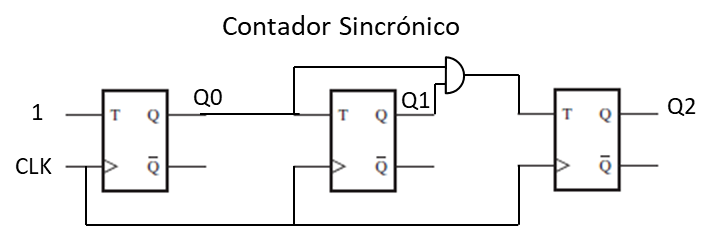
\includegraphics{../7-Async-Sync-Counter/contador sinc.png}

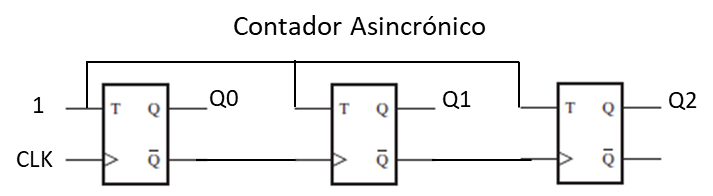
\includegraphics{../7-Async-Sync-Counter/contador asinc.png}

\subsection{Análisis de Ambos Circuitos}

Para poder analizar ambos circuitos, se implementó el circuito en una placa impresa (PCB) y se hizo uso de leds para hacer el circutio más interactivo.
A continuación se muestra el circuito en físico:
\begin{center}
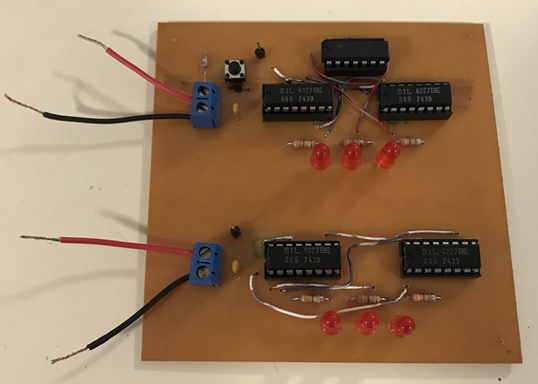
\includegraphics{../7-Async-Sync-Counter/pcb.png}
\end{center}
\chapter{Ultrasonido}
\subsection{Objetivo}
Implementar un circuito capaz de hacer mediciones de distancia con un sensor ultrasonico HC-SR04 (diseñado para ser usado en Arduino) sin el uso de ningún tipo de logica programable.
\subsection{Analisis}
Para poder empezar con el proceso de diseño se analizaron todas las etapas por las que deberian viajar las señales con el fin de realizar lo pedido.
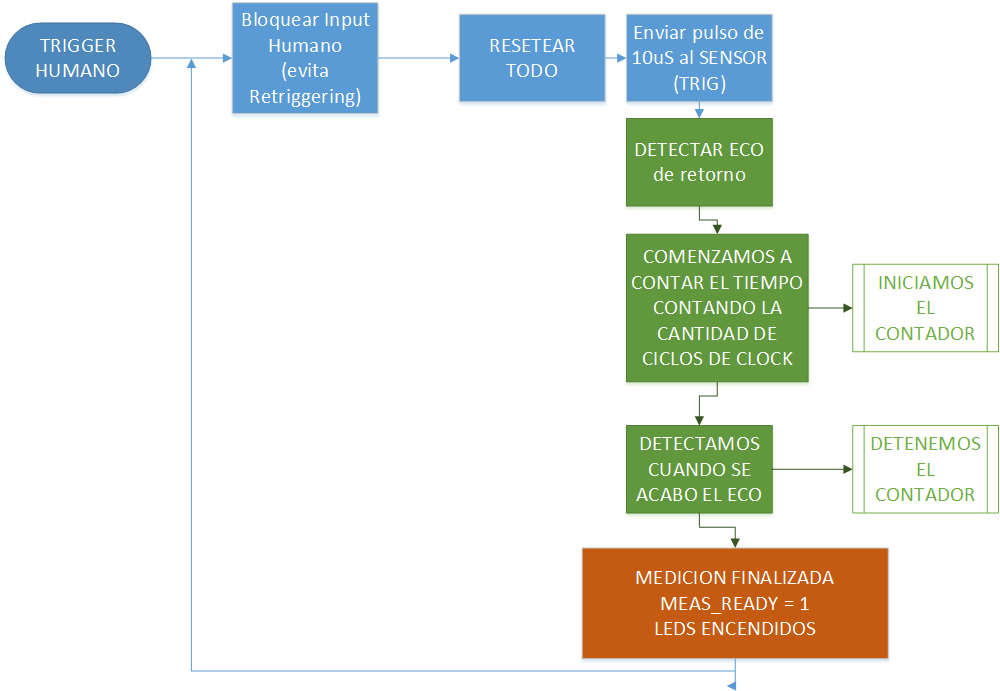
\includegraphics[scale=1]{../8-UltraSound/Driagrama-de-Flujo.png}
Dado que estamos trabajando con compuertas logicas fue bastante razonable pensar que en algún punto del diseño
\textbf{•}
\clearpage
\section*{Appendix}
\addcontentsline{toc}{chapter}{Appendix}


\begin{thebibliography}{}
\addcontentsline{toc}{chapter}{References}
\bibitem{INT1} Yoda. "A Brief History of Jedism" Journal of The New Jedi Order (Year): 93-98.
 \end{thebibliography} 
\end{document}